% Agent pipeline diagram (Figure in Section 4.2). Build with
%   pdflatex fig_agent_pipeline.tex
% Colors are the paper's reference palette only.
\documentclass[10pt]{standalone}
\usepackage{times}
\usepackage{amsmath}
\usepackage{tikz}
\usetikzlibrary{arrows.meta,positioning,shadows,calc}

% Only the reference palette, plus black text and white.
\definecolor{wbTeal}{HTML}{107A83}       % ref 1
\definecolor{wbTealLight}{HTML}{7DB7BE}
\definecolor{wbTerracotta}{HTML}{C36D56}
\definecolor{wbTerracottaLight}{HTML}{E1B2A8}
\definecolor{wbNavy}{HTML}{004E85}
\definecolor{wbNavyLight}{HTML}{7EA4C2}
\definecolor{wbOchre}{HTML}{DF8932}
\definecolor{wbOchreLight}{HTML}{E6C08C}
\definecolor{wbMaroon}{HTML}{8F1F22}
\definecolor{wbCream}{HTML}{F5DDB5}      % ref 2
\definecolor{wbMauve}{HTML}{CEA2B5}
\definecolor{wbLavender}{HTML}{9A9AB9}
\definecolor{wbIndigo}{HTML}{56669E}
\definecolor{wbAqua}{HTML}{50B9AE}

\tikzset{
  box/.style={rounded corners=2.5pt,align=center,inner xsep=3pt,inner ysep=2pt,
    font=\scriptsize,text=black,line width=.6pt},
  fillbox/.style={box,fill=#1,draw=#1},
  chip/.style={box,font=\scriptsize\bfseries,inner ysep=.8pt,inner xsep=2.5pt,minimum height=.34cm},
  step/.style={box,fill=#1,align=flush left,anchor=north west,inner ysep=2.5pt},
  arr/.style={-{Stealth[length=4pt,width=3.4pt]},line width=.7pt,draw=black},
  frame/.style={rounded corners=5pt,draw=wbLavender,line width=.7pt},
  lane/.style={rounded corners=3pt,draw=#1,line width=.6pt},
  note/.style={font=\scriptsize\itshape,text=black},
  title/.style={font=\footnotesize\bfseries,text=black},
  cards/.style={copy shadow={shadow xshift=3.6pt,shadow yshift=3.6pt,fill=wbTerracottaLight,draw=wbTerracotta},
    copy shadow={shadow xshift=2.4pt,shadow yshift=2.4pt,fill=wbTerracottaLight,draw=wbTerracotta},
    copy shadow={shadow xshift=1.2pt,shadow yshift=1.2pt,fill=wbTerracottaLight,draw=wbTerracotta}},
}

\begin{document}
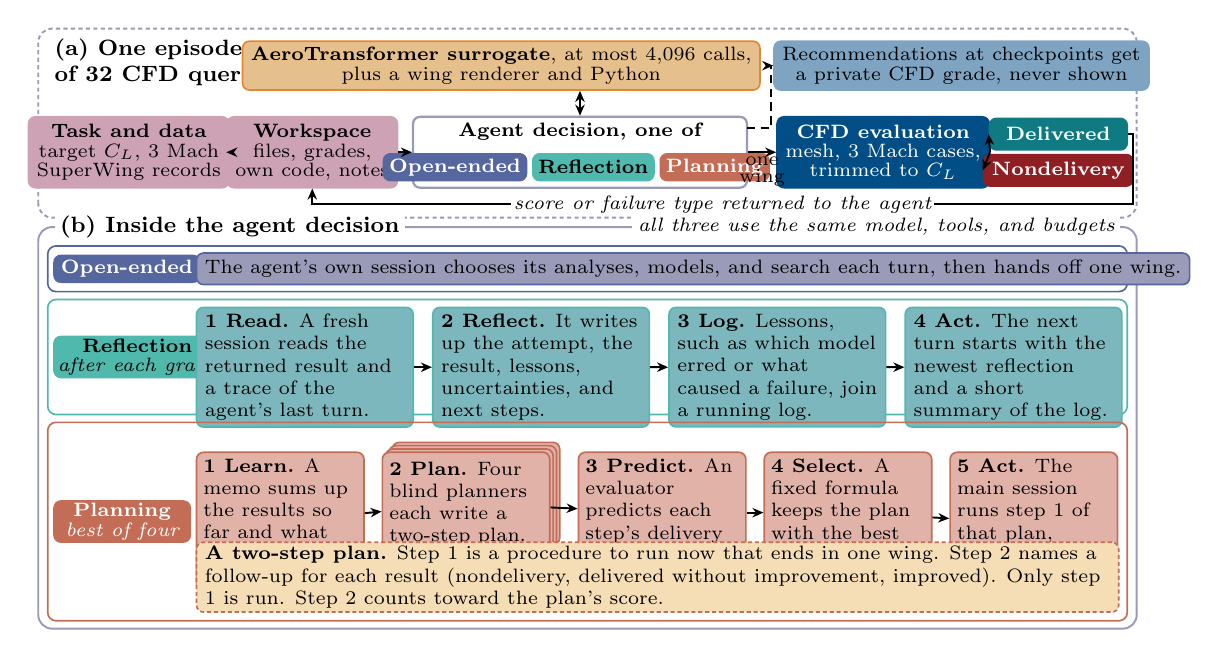
\begin{tikzpicture}[x=1cm,y=1cm]

% =====================================================================
% (a) One episode, y 5.22-7.62.  Main row at y=6.05, top row at y=7.15.
% columns: task 0.1-2.2 | ws 2.47-4.49 | dec 4.76-9.0 | cfd 9.62-11.84 | out 12.08-13.83
% =====================================================================
\draw[frame,dash pattern=on 1.5pt off 1.2pt] (0,5.22) rectangle (13.95,7.62);
\node[title,anchor=north west,align=left,inner sep=0pt] at (.2,7.5)
  {(a) One episode\\of 32 CFD queries};

\node[fillbox=wbMauve,minimum width=2.1cm,minimum height=.9cm] (task) at (1.15,6.05)
  {\textbf{Task and data}\\[-1pt]target $C_L$, 3 Mach\\[-1pt]SuperWing records};
\node[fillbox=wbMauve,minimum width=2.02cm,minimum height=.9cm] (ws) at (3.48,6.05)
  {\textbf{Workspace}\\[-1pt]files, grades,\\[-1pt]own code, notes};
\draw[arr] (task) -- (ws);

\node[fillbox=wbOchreLight,draw=wbOchre,minimum width=6.0cm,minimum height=.62cm] (tools) at (5.88,7.15)
  {\textbf{AeroTransformer surrogate}, at most 4,096 calls,\\[-1pt]plus a wing renderer and Python};
\node[box,fill=white,draw=wbLavender,line width=.8pt,minimum width=4.24cm,minimum height=.9cm]
  (dec) at (6.88,6.05) {};
\node[font=\scriptsize\bfseries,anchor=north,inner sep=2.5pt] at (dec.north) {Agent decision, one of};
\node[chip,inner xsep=2pt,fill=wbAqua,draw=wbAqua] (kb) at (7.05,5.86) {Reflection};
\node[chip,inner xsep=2pt,fill=wbIndigo,draw=wbIndigo,text=white,left=.06cm of kb] (ka) {Open-ended};
\node[chip,inner xsep=2pt,fill=wbTerracotta,draw=wbTerracotta,text=white,right=.06cm of kb] (kc) {Planning};
\draw[arr] (ws) -- (dec);
\draw[arr,{Stealth[length=4pt,width=3.4pt]}-{Stealth[length=4pt,width=3.4pt]}]
  (tools.south -| dec.north) -- (dec.north);

\node[fillbox=wbNavy,text=white,minimum width=2.22cm,minimum height=.9cm] (cfd) at (10.73,6.05)
  {\textbf{CFD evaluation}\\[-1pt]mesh, 3 Mach cases,\\[-1pt]trimmed to $C_L$};
\draw[arr] (dec) -- node[below,font=\scriptsize,inner sep=1.5pt,align=center] {one\\[-2pt]wing} (cfd);
\node[fillbox=wbTeal,text=white,font=\scriptsize\bfseries,minimum width=1.75cm,minimum height=.4cm,inner ysep=1pt]
  (ok) at (12.955,6.28) {Delivered};
\node[fillbox=wbMaroon,text=white,font=\scriptsize\bfseries,minimum width=1.75cm,minimum height=.4cm,inner ysep=1pt]
  (bad) at (12.955,5.82) {Nondelivery};
\draw[arr] (cfd.east) -- (ok.west);
\draw[arr] (cfd.east) -- (bad.west);
\draw[line width=.7pt] (ok.east) -- (13.9,6.28) -- (13.9,5.82) (bad.east) -- (13.9,5.82);
\draw[arr] (13.9,5.82) |- (3.48,5.39) node[pos=.75,fill=white,inner sep=1pt,note]
  {score or failure type returned to the agent} -- (ws.south);

\node[fillbox=wbNavyLight,minimum width=4.21cm,minimum height=.62cm] (priv) at (11.725,7.15)
  {Recommendations at checkpoints get\\[-1pt]a private CFD grade, never shown};
\draw[arr,densely dashed] (9.0,6.36) -- (9.31,6.36) |- (priv.west);

% =====================================================================
% (b) Inside the agent decision, y 0-5.1.  method chips 0.19-1.94, content 2.0-13.78
% =====================================================================
\draw[frame] (0,0) rectangle (13.95,5.1);
\node[title,anchor=west,fill=white,inner sep=2pt] at (.2,5.1) {(b) Inside the agent decision};
\node[note,anchor=east,fill=white,inner sep=2pt] at (13.75,5.1)
  {all three use the same model, tools, and budgets};

% ---- Lane A ----
\draw[lane=wbIndigo] (.12,4.28) rectangle (13.83,4.86);
\node[chip,fill=wbIndigo,draw=wbIndigo,text=white,minimum width=1.73cm,anchor=west] at (.19,4.57) {Open-ended};
\node[fillbox=wbLavender,draw=wbIndigo,anchor=west,minimum width=11.73cm,minimum height=.4cm,inner ysep=1pt]
  (a1) at (2.0,4.57)
  {The agent's own session chooses its analyses, models, and search each turn, then hands off one wing.};

% ---- Lane B ----
\draw[lane=wbAqua] (.12,2.72) rectangle (13.83,4.18);
\node[chip,fill=wbAqua,draw=wbAqua,inner xsep=1.25pt,minimum width=1.73cm,align=center,anchor=west] at (.19,3.45)
  {Reflection\\[-1pt]\normalfont\itshape after each grade};
\foreach \n/\x/\t in {
  b1/2.0/{\textbf{1 Read.} A fresh session reads the returned result and a trace of the agent's last turn.},
  b2/5.0/{\textbf{2 Reflect.} It writes up the attempt, the result, lessons, uncertainties, and next steps.},
  b3/8.0/{\textbf{3 Log.} Lessons, such as which model erred or what caused a failure, join a running log.},
  b4/11.0/{\textbf{4 Act.} The next turn starts with the newest reflection and a short summary of the log.}}
  \node[step=wbTealLight,draw=wbAqua,text width=2.54cm,minimum height=1.28cm] (\n) at (\x,4.09) {\t};
\draw[arr] (b1) -- (b2);
\draw[arr] (b2) -- (b3);
\draw[arr] (b3) -- (b4);

% ---- Lane C ----
\draw[lane=wbTerracotta] (.12,.1) rectangle (13.83,2.62);
\node[chip,fill=wbTerracotta,draw=wbTerracotta,text=white,minimum width=1.73cm,align=center,anchor=west] at (.19,1.36)
  {Planning\\[-1pt]\normalfont\itshape best of four};
\foreach \n/\x/\t in {
  c1/2.0/{\textbf{1 Learn.} A memo sums up the results so far and what seems to deliver.},
  c3/6.85/{\textbf{3 Predict.} An evaluator predicts each step's delivery and $L/D$.},
  c4/9.21/{\textbf{4 Select.} A fixed formula keeps the plan with the best expected $L/D$.},
  c5/11.57/{\textbf{5 Act.} The main session runs step 1 of that plan, handing off a wing.}}
  \node[step=wbTerracottaLight,draw=wbTerracotta,inner xsep=2.5pt,text width=1.95cm,minimum height=1.3cm] (\n) at (\x,2.25) {\t};
\node[step=wbTerracottaLight,draw=wbTerracotta,cards,inner xsep=2.5pt,text width=1.95cm,minimum height=1.3cm] (c2) at (4.36,2.25)
  {\textbf{2 Plan.} Four blind planners each write a two-step plan.};
\draw[arr] (c1) -- (c2);
\draw[arr] (c2) -- (c3);
\draw[arr] (c3) -- (c4);
\draw[arr] (c4) -- (c5);
\node[box,fill=wbCream,draw=wbTerracotta,dash pattern=on 1.5pt off 1pt,anchor=south west,
      text width=11.5cm,align=flush left,inner ysep=1.5pt] (plan) at (2.0,.2)
  {\textbf{A two-step plan.} Step 1 is a procedure to run now that ends in one wing. Step 2 names a follow-up
   for each result (nondelivery, delivered without improvement, improved). Only step 1 is run.
   Step 2 counts toward the plan's score.};

\end{tikzpicture}
\end{document}
